% siminos/spatiotemp/chapter/KStimeInt.tex
% $Author: predrag $ $Date: 2019-09-22 00:02:44 -0400 (Sun, 22 Sep 2019) $

% called by
%           siminos/spatiotemp/chapter/spatiotemp.tex
%           siminos/tiles/GuBuCv17.tex

%\section{Spatially periodic \KS}
%\label{sect:KStimeInt}

%    \PCedit{
%[{\bf 2016-02-06 Predrag}
%summarize the standard case on spatially $\speriod{}$-periodic domain]
%    }

It is not possible to integrate numerically the \KSe\ on the
\spt ly doubly infinite domain \refeq{e-ks}. Instead, the standard practice
is to confine the system to a spatially \speriod{}-periodic domain,
specify a smooth spatially periodic initial condition
$u(\conf,\zeit)=u(\conf+\speriod{},\zeit)$, and integrate
\beq
    u_\zeit + u_{\conf \conf} + u_{\conf \conf \conf \conf} + u_\conf u = 0
    \,,\quad
    x \in [0,\speriod{})
    \label{e-ksL}
\eeq
forward in time on the \spt\ cylinder of  \reffig{fig:spaceTime1}\,(a).
Though stable periodic solutions do exist\rf{FSTks86}, for a  generic,
sufficiently
large spatial domains, all numerical \KS\ solutions exhibit ``steady
state turbulence'' illustrated by \reffig{f:ks_largeL}.

%%%%%%%%%%%%%%%%%%%%%%%%%%%%%%%%%%%%%%%%%%%%%%%%%%%%%%
\begin{figure}[h]
    \begin{center}
\begin{minipage}[height=.20\textheight]{.18\textwidth}
\centering
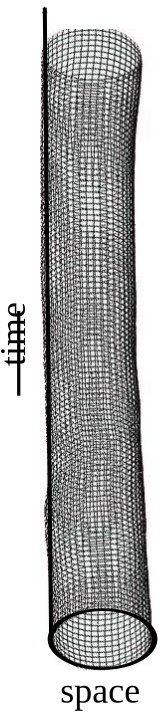
\includegraphics[width=.75\textwidth]{cylinderTime1}
    \vfill
\small{\texttt{(a)}}
\end{minipage}
~~~~
\begin{minipage}[height=.20\textheight]{.75\textwidth}
\centering
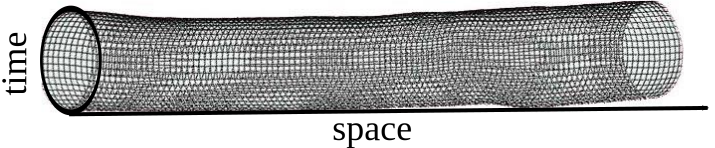
\includegraphics[width=.80\textwidth]{cylinderSpace1}
\\
\small{\texttt{(b)}}
\\
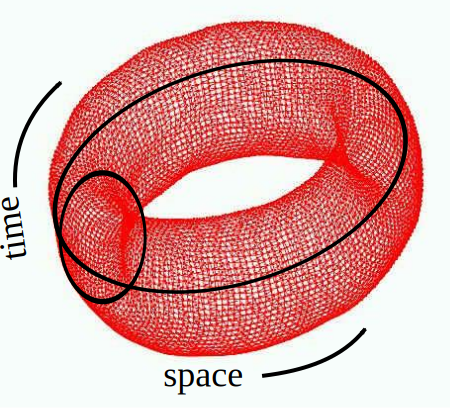
\includegraphics[width=.50\textwidth]{spaceTime1}
\\
\small{\texttt{(c)}}
\end{minipage}
    \end{center}
\caption{\label{fig:spaceTime1}
(a) The 1D \KSe\ is usually integrated on a \spt\ cylinder of an
    arbitrary fixed $\speriod{}$ periodic spatial extent, with time
    $\zeit\in\{-\infty,\infty)$; for an example, see \reffig{f:ks_largeL}.
(b) It is also possible to integrate the equation on a \spt\ cylinder of an
    arbitrary fixed $\period{}$ periodic temporal extent, with position
    ranging over $\conf\in\{-\infty,\infty)$, see \refsect{sect:KSspaceInt}.
(c) Here we shall seek {\spt}ly \twot\ solutions $u(\conf,\zeit)$ over a 2-torus of
    dynamically determined size $(\speriod{},\period{})$ , see
    \refsect{sect:KStwots}.
}
\end{figure}
%%%%%%%%%%%%%%%%%%%%%%%%%%%%%%%%%%%%%%%%%%%%%%%%%%%%%%


Smooth, spatially periodic velocity field $u$ %(\conf,\zeit)=u(x+\speriod{},\zeit)$
is naturally represented in the Fourier space,
\beq
  u(\conf,\zeit)
   =\sum_{m=-\infty}^{+\infty} a_m(\zeit)\,e^{ i 2\pi m\conf /\speriod{} }
\,,
\ee{eq:ksexp}
with the $1$D PDE \refeq{e-ksL}
replaced by an infinite set of
ODEs for the complex Fourier coefficients $a_m(t)$:
\beq
\dot{a}_m %= \pVeloc_m(a)
     = ( q_m^2 - q_m^4 )\, a_m
    - i \frac{q_m}{2} \sum_{k=-\infty}^{+\infty} a_k a_{m-k}
\ee{SCD07:expan}
where $q_m =  2\pi m/\speriod{}$.
Since $u(\conf,\zeit)$ is real, $a_m=a_{-mm}^\ast$, and we can replace the
sum by a $m > 0$ sum.


Consider the \KSe\ \refeq{e-ks} on a {\spt} cylinder
$(\conf,\zeit)\in([0,\speriod{}),\reals)$, defined on a a spatial strip of width
$\speriod{}$, with spatially periodic boundary condition $u(\conf,\zeit)=u(x+\speriod{},t)$, see
\reffig{fig:spaceTime1}\,(a).
Discretize spatially the \KS\ system by Fourier expanding the field
$u(\conf_n,\zeit)= u_n(\zeit)$ over $N$ points of a periodic spatial 1D
lattice $\conf_n=n\speriod{}/N$,
\bea
  \Fu_k(\zeit) &=& \frac{1}{N} \sum^{N-1}_0 u_n(\zeit) e^{-iq_k\conf_n}
  \,=\, \frac{1}{N} \sum^{N-1}_0 u_n(\zeit) e^{-i 2 \pi k n /N}
  \,,\quad
q_k = \frac{2 \pi k}{\speriod{}}
\continue
  u_n(\zeit) &=&\sum_{k=0}^{N-1}\Fu_k(\zeit) e^{iq_k\conf_n}
    \,=\, \sum_{k=0}^{N-1}\Fu_k(\zeit) e^{i 2 \pi k n /N}
\,,
\label{spatFT}
\eea
and expressing \refeq{e-ks} in terms of discrete spatial Fourier modes as
$N$ ordinary differential equations (ODEs) in time
\beq
%\dot{\Fu}_k(\zeit)
\frac{d~}{d\zeit}\Fu_k(\zeit)
= ( q_k^2 - q_k^4 )\, \Fu_k(\zeit)
- \frac{i q_k}{2} \!\sum_{k'=0}^{N-1} \!\!\Fu_{k'}(\zeit) \Fu_{k-k'}(\zeit)
\,.
\label{e-Fks}
\eeq

        \PCedit{
In the Fourier representation the \reqva\ time dependence is
\beq
 a_k(t) e^{-itc q_k} = a_k(0)
\,.
\ee{reqvaF}
Differentiating with respect to time, we obtain
the Fourier space version of the \reqv\ condition
\refeq{KSeqvCond},
\beq
 \pVeloc_k(a) - i q_k c a_k = 0
\,,
\ee{reqvCondF}
which we solve for (time independent) $a_k$ and $c$.
        }


%%%%%%%%%%%%%%%%%%%%%%%%%%%%%%%%%%%%%%%%%%%%%%%%%%%%%%%%%%%%%%%%%%
\subsubsection{Temporal stability}
\label{exam:KurSivTempstab}
% From ChaosBook Chapter{PDEs}{2016-01-23}{Turbulence?}

To calculate the temporal stability of a spatial \eqv\ $\Fu_\stagn$
    \PC{2019-05-16}{dropped
(or a temporally \po).
%\refeq{eq:StabMat} is plain wrong, no?
    }
we need to evaluate  the \stabmat\ (the matrix of temporal
velocity gradients)
\beq
%  \Mvar_{ij}(a_q)  = \left.\frac{\partial v_i}{\partial a_j}\right|_{a=a_q}
  \Mvar_{ij}(\Fu_\stagn)  =
  \left.\frac{\partial \dot{\Fu}_i}{\partial \Fu_j}\right|_{\Fu={\Fu_\stagn}}
\,.
\label{eq:StabMat}
\eeq
For \KS\ we can
compute $\Mvar(\Fu_q)$ efficiently using the linearity
of the Fourier transform, see \refref{SCD07}.
Consider the four matrices
$\frac{\partial \dot{b}_k}{\partial b_j},\frac{\partial
\dot{b}_k}{\partial c_j},\frac{\partial \dot{c}_k}{\partial
b_j},\frac{\partial \dot{c}_k}{\partial c_j}$,
where the real and imaginary parts of $\Fu_k$ are
$\Fu_k=b_k+ic_k$.
For illustration, consider the $b_k=0$ invariant antisymmetric subspace
$\bbU^+$,
\beq
\dot{c}_k= \pVeloc_k(c)
     = ( q_k^2 - q_k^4 )\, a_k
    - \frac{q_k}{2} \sum_{m=-\infty}^{\infty} c_m c_{k-m}
\,,\qquad   q_k = k/2\pi \speriod{}
\,.
\ee{expan}
The temporal {\stabmat} \refeq{eq:StabMat} restricted to the invariant
antisymmetric subspace $\bbU^+$ follows from \refeq{expan}:
\beq
{\Mvar}_{kj}(c) =\frac{\pde v_k(a)}{\pde c_j  }
=(q_k^2- q_k^4)\delta_{kj} + q_k ( c_{k-j}- c_{k+j})
\,.
\ee{expanMvar}
For the full \statesp, consult sect.~6.2 {\em Calculating stability of equilibria}
of Siminos thesis\rf{SiminosThesis}.

\subsubsection{\KS\ $u=0$ temporal equilibrium}
\label{sect:KSu0equiT}

The \KS\ flat flame front $u(\conf,\zeit)=0$ is always a temporal {\eqv} of \refeq{e-ks},
whose temporal {\stabmat} \refeq{expan} is
diagonal, with real temporal stability exponents $\eigExp[k]= q_k^2- q_k^4$,
the eigenvectors are spatial Fourier modes, and consequently the
temporal {\jacobianM} is diagonal as well,
\(
\jMps^t_{kj} = \delta_{kj} \ExpaEig_k(\zeit)
    \,,\;
\ExpaEig_k(\zeit) = e^{(q_k^2- q_k^4)\,t}
\,.
\)
%	} %end \example{\Stabmat,  antisymme
%%%%%%%%%%%%%%%%%%%%%%%%%%%%%%%%%%%%%%%%%%%%%%%%%%%%%%%%%%%%%%%%%%
